\section{Servizi di un Sistema Operativo}
    Un sistema operativo fornisce un ambiente in cui eseguire programmi e fornire servizi, che possono variare in base allo specifico sistema operativo, ma possiamo riconoscere alcune classi comuni di servizi.
    
    \subsection{Funzionalità utili all'utente}
        Un primo insieme di servizi offre funzionalità utili all'utente.
        
        \paragraph{Interfaccia con l'utente.} O UI, può assumere diverse forme. La più comune consiste di un'interfaccia a finestre con un puntatore e un input testuale, ma per dispositivi come tablet e smartphone possiamo avere touch screen con relativi metodi di interazione. Possiamo anche avere un'interfaccia a linea di comando (CLI).
        
        \paragraph{Esecuzione di un programma.} Un sistema operativo deve permettere di caricare in memoria ed eseguire un programma. Deve anche poter terminare l'esecuzione in maniera corretta o anomala (segnalando quest'ultimo caso).
        
        \paragraph{Operazioni di I/O.} Un programma in esecuzione dovrebbe poter richiedere operazioni di I/O, che per alcuni dispositivi potrebbero richiedere funzioni particolari. Inoltre per motivi di efficienza e protezione, l'utente non può controllare direttamente questi dispositivi, quindi il sistema operativo deve mettere a disposizione strumenti adeguati per la loro gestione.
        
        \paragraph{Gestione del file system.} I programmi richiedono l'esecuzione di operazioni di lettura e scrittura su file, possono modificarli, cercarli o cancellarli, oltre che gestire directory. Alcuni sistemi forniscono tutte o alcune di queste operazioni in base alla proprietà dello stesso, mentre molti sistemi operativi fanno scegliere all'utente diversi file system con funzionalità e prestazioni specifiche.
        
        \paragraph{Comunicazioni.} Spesso un processo ha bisogno di scambiare informazioni con un altro processo in esecuzione. Questo può avvenire fra processi sullo stesso calcolatore o attraverso la rete. Questo scambio può avvenire tramite una \textbf{memoria condivisa}, che permette a entrambi di leggere e scrivere in una porzione di memoria che condividono, o attraverso lo \textbf{scambio di messaggi}, cosa gestita dal sistema operativo.
        
        \paragraph{Rilevamento di errori.} Il sistema operativo deve essere capace di gestire diversi tipi di errore, come un fallimento dell'hardware, un problema nei dispositivi di I/O o nei programmi utente. A volte l'unico modo di gestire correttamente queste situazioni è arrestare il sistema, mentre altre volte potrebbe essere necessario solo arrestare il processo colpevole o inviare un messaggio di errore.
        
    \subsection{Funzioni utili al sistema}
        Un secondo insieme comprende funzioni che assicurano il corretto funzionamento del sistema, anche se non sono direttamente rilevate dall'utente.
        
        \paragraph{Allocazione delle risorse.} Se più utenti usano la stessa macchina (situazione ormai rara) o più processi sono in esecuzione contemporaneamente, è compito del sistema operativo gestire le risorse in modo che nessun processo monopolizzi la potenza computazionale e nessuno muoia per mancanza di risorse.
        
        \paragraph{Logging.} È in pratica il mantenere traccia di quali programmi o processi consumano quante risorse, e altre informazioni affini. Questo può servire per una serie di cose, fra cui compilare statistiche che possono essere utili a una futura gestione più efficiente del sistema.
        
        \paragraph{Protezione e sicurezza.} La \textbf{protezione} assicura che l'accesso alle risorse del sistema sia controllato, in maniera che nessun estraneo possa accedervi. La \textbf{sicurezza} inizia dalla richiesta di autenticazione e si espande fino al controllo di accessi maligni tramite dispositivi di I/O. Un sistema protetto e sicuro deve porre precauzioni ovunque, in quanto la forza di una catena è solo quella del suo anello più debole.
        
\section{System Calls (chiamate di sistema)}
    Le chiamate di sistema rappresentano un'interfaccia per i servizi resi disponibili dal sistema operativo. Esse sono il principale metodo di interazione fra i programmi utenti e il kernel, in quanto spesso vengono usate durante la modalità utente per richiedere servizi disponibili solo in modalità kernel.
    
    I programmatori spesso non accedono direttamente nemmeno alle system calls, ma hanno a disposizione una \textbf{API} (\textit{application programming interface}), che varia da sistema a sistema (Windows ha le sue API, mentre i sistemi basati sullo standard POSIX, il che comprende praticamente tutti i sistemi UNIX, Linux e macOS, hanno la loro per esempio), e che chiama le system calls corrette richieste dall'utente. Ci sono una serie di ragioni per cui uno sviluppatore potrebbe preferire l'utilizzo delle API, come per esempio rendere l'applicazione portabile su tutti i sistemi operativi che operano sullo stesso standard.
    
    Le system calls vengono richiamate tramite un codice identificativo unico per ognuna e sono memorizzate in una tabella.
    
    \subsection{Categorie di system calls}
        Le system calls possono essere classificabili in approssimativamente sei categorie, che andremo di seguito a descrivere.
        
        \paragraph{Controllo dei processi.} Ci sono molti punti di vista sotto cui i processi devono essere gestiti; la loro interruzione per esempio, può essere regolare o anomala, e un'interruzione non andata a buon fine ha diversi livelli di gravità (possiamo generalizzare il concetto dicendo che un'interruzione andata a buon fine ha livello di gravità 0). Quando un processo viene terminato in maniera anomala potremmo voler analizzare dati relativi alla sua terminazione.
        
        Un'altra caratteristica dei processi è ovviamente la loro creazione, quante risorse consuma e per quanto tempo viene eseguito. Inoltre, in un processore multitask abbiamo bisogno di gestire il parallelismo, schedulando l'esecuzione e l'arresto dei vari processi in base alla disponibilità del processore.
        
        Tutte queste operazioni vengono gestite tramite chiamate di sistema.
        
        \paragraph{Gestione dei file.} In base al file system devono essere rese disponibili determinate operazioni sui file, fra cui creazione, rimozione, apertura, lettura, scrittura, chiusura, eccetera. Le stesse operazioni, nel caso in cui il file system sia strutturato in directories, devono essere disponibili anche sulle suddette. Il sistema operativo potrebbe rendere disponibili queste operazioni tramite chiamate di sistema, interfacce grafiche, programmi, etc.
        
        \paragraph{Gestione dei dispositivi.} L'assegnamento e in generale la gestione delle risorse avviene spesso tramite dispositivi: la memoria viene assegnata tramite il disco, la potenza di calcolo tramite il processore, le elaborazioni grafiche tramite la GPU, etc.
        
        È quindi ovvio che c'è bisogno di un modo per gestire questi dispositivi. Questi devono essere, nel caso di un sistema multiutente per esempio, assegnati talvolta a un utente in maniera esclusiva, inizializzati, chiusi quando necessario. Queste operazioni possono essere viste come simili a quelle eseguite sui file, e difatti alcuni sistema operativi, come Linux, uniscono la gestione dei file e dei dispositivi in un unico sistema file-dispositivi.
        
        \paragraph{Gestione delle informazioni.} Una buona parte delle chiamate di sistema serve a scambiare informazioni fra il sistema e l'utente. Ci sono molte informazioni che l'utente potrebbe voler recuperare dal sistema, come la data, l'ora, o informazioni specifiche sulla memoria. O ancora, informazioni sui processi, di cui il sistema tiene traccia in maniera dettagliata, descrivendone per esempio il tempo di esecuzione e le risorse utilizzate.
        
        \paragraph{Comunicazione.} Ci sono due metodi molto diffusi di scambio di messaggi fra processi. Il primo è il \textbf{modello a messaggi}, che prevede lo scambio di messaggi sia in maniera diretta che indiretta, tramite l'utilizzo di una \textit{mailbox} comune. Il processo che fornisce il messaggio si chiama \textit{client}, mentre quello che lo riceve si chiama \textit{server}.
        
        L'altro metodo per scambiare i messaggi è usare una \textbf{memoria condivisa}, che prevede la lettura e la scrittura da parte di due processi sulla stessa memoria, con la condizione di evitare conflitti (non scrivere contemporaneamente). Questo avviene per esempio con i \textit{thread}.
        
        Lo scambio di messaggi è preferibile quando vanno scambiate piccole quantità di informazioni e quando i due processi esistono su calcolatori distinti, per esempio che comunicano tramite la rete, mentre l'accesso condiviso alla memoria permette la massima velocità ed è quindi preferibile per grandi scambi di dati.
        
        \paragraph{Protezione.} Storicamente era necessario tenere in considerazione la protezione su sistemi che prevedevano l'utilizzo da parte di molti utenti, ma oggi, con l'accesso di ogni dispositivo a Internet, è necessario prendere sempre in considerazione la protezione.
        
        Il sistema operativo può chiedere i permessi e l'autenticazione all'utente e di conseguenza permettere o negare l'accesso.
        
\section{Struttura del sistema operativo}
    Allo scopo di far funzionare correttamente un sistema complesso come un sistema operativo moderno e di non renderne impossibile la manutenzione, è necessario strutturarne le componenti in maniera studiata. Un metodo di strutturazione è quello \textbf{monolitico}, che tuttavia col tempo è stato abbandonato in favore di una struttura \textbf{modulare}, che prevede la presenza di moduli con interfacce ben definite.
    
    \subsection{Struttura monolitica}
        Il modo più semplice di strutturare un sistema operativo è tramite l'assenza di struttura, ossia mettendo tutte le funzionalità del kernel in un unico file binario che viene eseguito una volta all'interno di un unico spazio di indirizzamento. Abbiamo per esempio il sistema operativo UNIX originale, che consta di due parti: il kernel e i programmi di sistema. Un sistema così strutturato è difficile da gestire, ma ottiene un vantaggio in termini di prestazioni in quanto il grande numero di servizi e funzioni eseguite all'interno del kernel implicano un overhead ridotto, e ciò giustifica alcuni elementi di questo tipo di struttura all'interno dei sistemi operativi moderni.
        
    \subsection{Approccio stratificato}
        I sistemi monolitici vengono anche chiamati \textbf{strettamente accoppiati} (\textit{tightly coupled}), in quanto ogni parte del kernel è dipendente da ogni altra parte. In alternativa possiamo pensare di strutturare il sistema con in mente un \textbf{basso accoppiamento} (\textit{loosely coupled}), il che ci permette di modificare un modulo senza andare necessariamente sugli altri.
        
        Un modo di rendere modulare un sistema operativo è tramite la \textbf{stratificazione}. In un tale sistema, gli strati più bassi rappresentano l'hardware, mentre quelli più alti l'interfaccia utente. 
        
        \begin{figure}
            \centering
            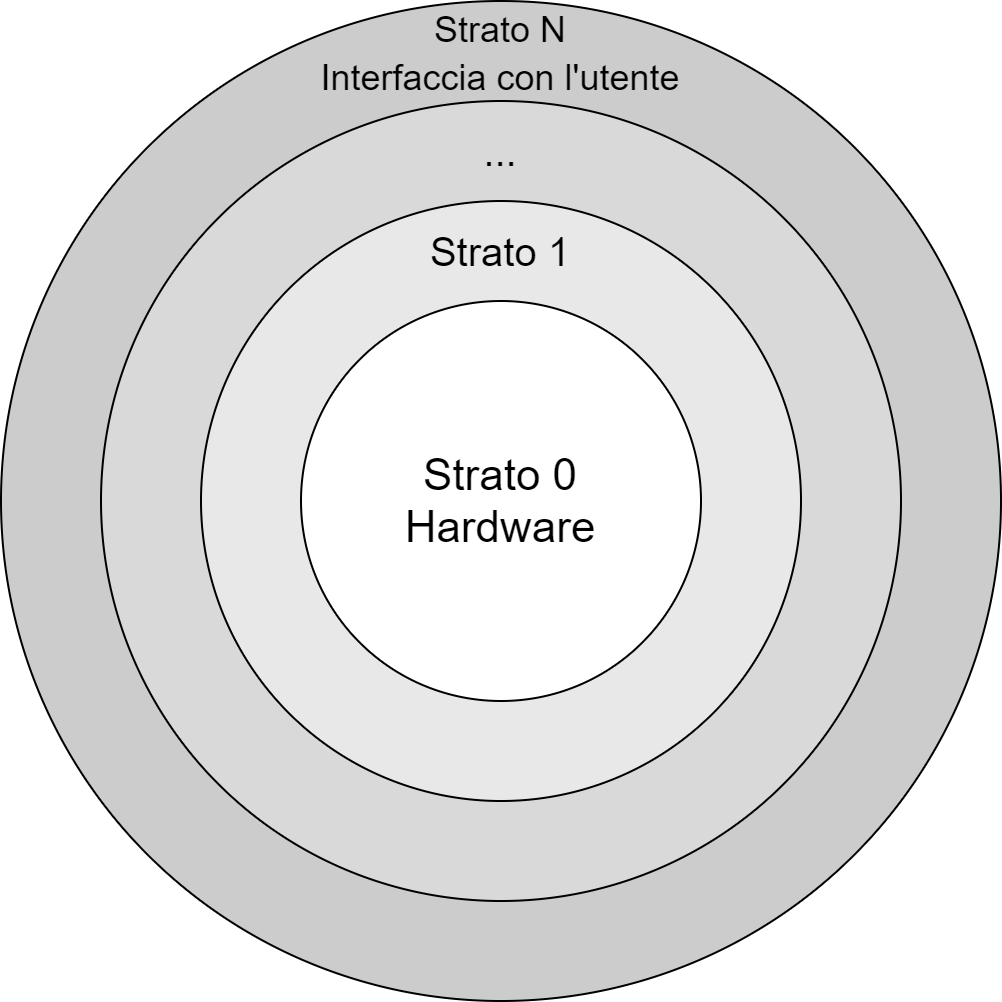
\includegraphics[width=0.5\textwidth]{img/img5.png}
            \caption{Struttura a strati di un sistema operativo.}
            \label{fig:img5}
        \end{figure}
        
        C'è da dire che recentemente si sono aggiunti strati addirittura superiori all'interfaccia utente. Pensiamo per esempio alle macchine virtuali, che hanno i loro strati, tutti superiori all'interfaccia utente, e forniscono anche loro un'interfaccia utente.
        
        Il funzionamento degli strati è opaco. Uno strato fornisce servizi allo strato superiore, e può richiederne a quello direttamente inferiore. Questo tipo di struttura rende relativamente facile la progettazione, in quanto possiamo sviluppare uno strato dando per scontato che quelli inferiori siano stati correttamente testati e usando le funzioni che ci mettono a disposizione. Questo metodo viene usato con successo per esempio nella costruzione di applicazioni web, ma raramente un approccio a stati puro viene osservato in un sistema operativo, in quanto è difficile definire le operazioni di un dato strato, e le prestazioni ne soffrono molto.
        
        La soluzione adottata spesso dai sistemi operativi moderni è un approccio ibrido, in cui abbiamo pochi strati con più funzioni nel singolo strato.
        
    \subsection{Microkernel}
        Come abbiamo visto in precedenza, il sistema operativo UNIX, in funzione della sua struttura monolitica, tendeva a crescere sempre di più, diventando sempre più difficile da gestire.
        
        Verso la metà degli anni '80 fu sviluppato il sistema operativo \textbf{Mach}, con il kernel strutturato in moduli secondo il cosiddetto orientamento a \textbf{microkernel}. La filosofia dietro questo tipo di strutturazione è quella di rimuovere dal kernel tutte le funzioni non strettamente necessarie, fornendole come programmi di livello utente e di sistema. Non c'è un consenso comune su quali servizi siano strettamente necessari, ma in generale un microkernel offre i servizi minimi di gestione dei processi, della memoria e della comunicazione. Ne risulta un microkernel di dimensioni molto ridotte e più facile da gestire a causa del grado di modularità introdotto.
        
        Lo scopo principale di un microkernel è quello di fornire funzioni di comunicazione fra i programmi client e i vari servizi, comunicazione che avviene tramite messaggi.
        
        Ovviamente un kernel di questo tipo è molto più facile da gestire, espandere ed è inoltre più sicuro, in quanto la compromissione di un servizio avviene spesso nello spazio utente, lasciando al sicuro le funzioni core del sistema operativo.
        
        Lo svantaggio è che i microkernel possono incorrere in cali di prestazioni, principalmente dovuto a un maggiore overhead causato dalla necessità di far comunicare due o più processi in spazi di indirizzamento diversi.
        
    \subsection{Moduli}
        Forse il miglior metodo attualmente disponibile per la progettazione di sistemi operativi si basa sull'utilizzo di \textbf{moduli del kernel caricabili dinamicamente}. In questo contesto il kernel è costituito da una serie di componenti di base che vengono poi integrati da funzionalità caricate dinamicamente all'avvio o durante l'esecuzione per mezzo di moduli. Molte implementazioni moderne di UNIX, come Linux, macOS e Solaris, come anche Windows, usano questo metodo.
        
        L'idea è che il kernel debba fornire alcuni servizi principali e offrire gli altri servizi in maniera dinamica, senza tuttavia aggiungerli direttamente al kernel, in quanto ciò richiederebbe una ricompilazione.
        
        Il risultato finale ricorda un sistema a strati, in quanto diverse sezioni del kernel offrono servizi ben distinti, ma ha una maggiore flessibilità (è meno opaco) in quanto ogni modulo può richiamare ogni altro modulo. Ricorda per certi versi anche l'approccio a microkernel, in quanto la parte principale del kernel implementa solo le funzioni di base, ma è più efficiente siccome i moduli caricati dinamicamente non devono comunicare tramite messaggi.
        
        Linux implementa un sistema di LKM, \textit{loadable kernel module}, principalmente per caricare driver di dispositivi e file system.
        
\section{Linker e Loader}
    Generalmente un programma risiede su un disco in forma di un file binario eseguibile. Per essere eseguito su una CPU, il programma deve essere caricato in memoria e inserito nel contesto di un processo.
    
    Innanzitutto i file sorgente vengono compilati in file oggetto progettati per essere ricaricati in qualsiasi locazione della memoria, e sono chiamati \textbf{file oggetto rilocabili}. In seguito, il \textit{linker} combinai file oggetto rilocabili in un singolo file binario eseguibile.
    
    Durante la fase di \textbf{linking}, possono essere inclusi altri file oggetto o librerie, dando a questa fase una natura che si presta a una certa modularità.
    
    Per caricare il file eseguibile in memoria, dove diventa idoneo e disponibile all'esecuzione, viene usato un \textbf{loader}. Una fase del caricamento è la rilocazione, la quale ha il compito di assegnare le locazioni di memoria definitive al programma, in modo da poter, per esempio, trovare le variabili globali e accedere alle funzioni di libreria.
    
    Ci sono molti standard per questo tipo di file, per esempio in ambiente Linux abbiamo il formato \textbf{ELF}, ossia Executable and Linkable Format. Oltre al codice macchina compilato e metadati relativi a simboli e funzioni, questo contiene anche un \textit{entry point}, che è semplicemente la prima istruzione da eseguire.